



\section{The Hardware Sampling Library: hws}

In the remainder of this thesis, I will focus mostly on the \textbf{walltime} and \textbf{efficiency} mainly with respect to the energy efficiency of the code examples when I talk about performance portability. 
Thereby, gathering basic \textbf{walltime} information is possible in a straightforward way with normal tools directly provided by \cpp, as shown in \autoref{code:walltime_measurement}.


However, gathering efficiency metrics like energy consumption, but also memory, or compute utilization poses more challenges, especially if we want to get this information in a vendor-independent way for NVIDIA, AMD, and Intel \glspl{gpu} and \glspl{cpu}. 
While all hardware vendors provide some form of gathering this information through custom libraries, collecting all this information in a vendor-independent way is far from trivial since these libraries do not agree to a standardized interface. 
As an example, to gather the total power consumption (since the last driver reload) for NVIDIA, AMD, and Intel \glspl{gpu}, the library functions shown in \autoref{code:vendor_labrier_calls} must be used.

\begin{listing}
    \begin{minted}{c++}
// NVML
unsigned long long power{};  // mJ
nvmlReturn_t errc = nvmlDeviceGetTotalEnergyConsumption(device_handle, &power);

// ROCm SMI library
[[maybe_unused]] std::uint64_t timestamp{};
float resolution{};
uint64_t power{};  // @$\mu$@J
rsmi_status_t errc = rsmi_dev_energy_count_get(device_handle, &power, &resolution, &timestamp);
float value = power * resolution;

// Level Zero
std::uint32_t num_power_domains{ 0 };  // @$\mu$@J
// enumerate all power domains
if (zesDeviceEnumPowerDomains(device_handle, &num_power_domains, nullptr) == ZE_RESULT_SUCCESS) {
    power_handles.resize(num_power_domains);
    if (zesDeviceEnumPowerDomains(device_handle, &num_power_domains, power_handles.data()) == ZE_RESULT_SUCCESS) {
        // we found at least one power domain (can be empty if reading power related counters isn't supported on the device)
        if (!power_handles.empty()) {
            // get the total power consumption of the first power domain
            zes_power_energy_counter_t energy_counter{};
            if (zesPowerGetEnergyCounter(power_handles.front(), &energy_counter) == ZE_RESULT_SUCCESS) {
                uint64_t power = energy_counter.energy;
            }
        }
    }
}
    \end{minted}
    \caption{
    Example library function calls to gather the total power consumption since the last driver reload from an NVIDIA \gls{gpu} using \gls{nvml}, an AMD \gls{gpu} using \gls{rocmsmi}, and Intel \gls{gpu} using Level Zero.
    Note that the respective environments must be initialized beforehand and that the \code{device_handle} points to a supported and available device.}
    \label{code:vendor_library_calls}
\end{listing}

\autoref{code:vendor_library_calls} shows too major problems in gathering such information in a vendor-independent way. 
First, as already mentioned, the \glspl{api} greatly differ between the different vendors. 
For example, using \gls{nvml} collecting the total power consumption can be done in two lines of code, when using Intel's Level Zero on the other hand, we at least need eight lines of code. 
Second, the libraries do not even agree to the same physical unit: While \gls{rocmsmi} and Level Zero both report the total power consumption in \si{\mu\joule}, NVIDIA's \gls{nvml} library reports it in \si{\milli\joule}.

An additional challenge is that for the walltime it may be sufficient to report it once to get the runtime of the whole application, but for, e.g., the energy consumption it is necessary to sample the information during the whole program execution to get more fine-grained information of your application. 

There already exist small and large libraries which solve at least some of these problems. 
However, they are all restricted in one or another way.
For example, the smaller libraries all support only a small subset of the possible hardware I am interested in. 
\cite{araf_verified_2020, leinardi_greenwithenvy_2024, noauthor_gpu_2024, guerreiro_gpgpu_2018} only support NVIDIA \glspl{gpu}, \cite{amd_amd_2024, noauthor_gpu_2023} only support AMD \glspl{gpu}, \cite{noauthor_ricks-lab_2024} supports NVIDIA and AMD \glspl{gpu}, \cite{benoit_courty_mlco2codecarbon_2024} supports NVIDIA and Intel \glspl{gpu}, \cite{noauthor_libgpucounters_2024} supports ARM Immortalis and Mali \glspl{gpu}, and \cite{google_hardwareperfcounter_2022} supports Adreno and Mali \glspl{gpu}.

The larger libraries do support more different hardware, but with one exception they also do not support all hardware I am interested in. 
PAPI~\cite{mucci_papi_1999} supports low-level performance counters to get various information from different \glspl{cpu} as well as NVIDIA and AMD \glspl{gpu}. 
Likwid~\cite{thomas_gruber_likwid_2023} is similar to PAPI in that it also supports low-level performance counters for different hardware. 
Its main focus lies on \glspl{cpu}, but NVIDIA and AMD \glspl{gpu} are also supported although officially only in an experimental state. 
The PowerAPI~\cite{fieni_powerapi_2024} is a collection of different tools that can be used to measure and analyze the power consumption of applications. 
It supports \glspl{cpu} and \glspl{gpu} from Intel and NVIDIA \glspl{gpu}. 
VARIORUM~\cite{noauthor_variorum_2024} is the only library that supports generic wrappers around low-level \gls{api} functions for all major \gls{cpu} and \gls{gpu} vendors. 

However, none of these libraries support sampling of hardware information during the whole programming execution. 
Therefore, I wrote my own hardware sampling library \textbf{hws} that also wraps the low-level functions from all major hardware vendors and additionally exposes an easy-to-use sampling interface to be able to automatically gather all necessary information during the whole program execution. 



\cite{breyer_hws_2024}
\cite{breyer_hardware-independent_2024} % poster

\begin{itemize}
    \item \cpp with Python bindings using Pybind11 \cite{jakob_pybind11_2017}
    % \item CPUs via trubostat, lscpu, free \cite{brown_turbostat_nodate, qian_lscpu_nodate, small_free_nodate}
    % \item NVIDIA GPUs via NVML \cite{nvidia_nvml_2024}
    % \item AMD GPUs via ROCM SMI lib \cite{amd_rocm_2024}
    % \item Intel GPUs via Level Zero \cite{intel_level_2024}
\end{itemize}

%\todo{restructure}


For better usability, I structured the hardware library such that the hardware samples are grouped into different categories. 
During the construction of a hardware sampler, these categories can be selectively disabled or enabled such that the user can determine what samples he really wants to collect.
The different sample categories are the following:
\begin{description}
    \item[general:]%
    The general category includes samples identifying the current hardware architecture, its name, or its current compute and/or memory utilization.
    \item[clock-related:]%
    The clock-related category is responsible for gathering samples related to any kind of clock also including memory clocks. 
    It stores minimum and maximum clock frequencies, as well as the running values gathered during sampling. 
    Additionally, information regarding hardware throttling and its reasons are gathered.
    \item[power-related:]%
    The power-related category gathers information like the power limit, the current power draw, or the total power consumption. 
    Note that on the \gls{cpu} the total power consumption is always calculated using an integral of the measured current power draws. 
    \item[memory-related:]%
    The memory-related category gathers information about the current main memory usage like total, free, and used memory, but also for \glspl{gpu} information about the used \gls{pcie} interconnect or for \glspl{cpu} information about the Cache hierarchy and sizes. 
    \item[temperature-related:] The temperature-related category gathers information about the current and maximum allowed temperatures, as well as potential fan information. 
    \item[gfx-related:] On \glspl{cpu} only, this category gathers i\gls{gpu} related information if an i\gls{gpu} is available. 
    \item[\enquote{idle states}:] Also on \glspl{gpu} only, this category saves the idle state information output by \textit{turbostat}.
\end{description}
For more information about all possible hardware samples for each category, including the sample name, its physical unit, and on which hardware it is supported, refer to the hws GitHub repository\footnote{\url{https://github.com/SC-SGS/hardware_sampling}}.

The general flow of the hws library looks as follows:
\begin{enumerate}
    \item%
    A new hardware sampler is constructed, initializing the required environment from the respective vendor library. 
    An atomic reference count is used to ensure that the respective environments are only initialized once. 
    Note that it is supported to start as many hardware samplers as one wishes and that combination of different hardware samplers is supported. 
    If everything should be sampled, it is easiest to use a \code{system_hardware_sampler}.
    \item%
    A hardware sampler is then started using the \code{start_sampling()} function which internally spawns a new \code{std::thread}. 
    The actual sampling process then takes place asynchronously in this newly created thread. 
    Note that one thread is created for each hardware sampler. 
    The \code{system_hardware_sampler} also starts as many threads as it encapsulates other hardware samplers. 
    \item%
    All supported hardware samples are initialized: The fixed samples to their final values and the running samples to their first value. 
    This step is also used to determine which hardware samples are supported on the current hardware. 
    All theoretically by hws supported samples are queried and if the respective vendor function returns with an error, i.e., a sample is not supported, the value will be set to an \code{std::nullopt} indicating that it can be ignored in future sampling attempts during the sampling loop. 
    \item%
    The actual sampling loop is started. 
    Here, a new value is added to every supported running sample. 
    At the end, the current thread sleeps for the amount of time specified by the sampling interval before it starts again to sample new values. 
    Using the \code{pause_sampling()} and \code{resume_sampling()} functions, the sampling of new values can temporarily be paused using an atomic flag as a signaling variable. 
    \item%
    At the end, one must call the \code{stop_sampling()} function which waits until the current sampling loop has finished and then joins on the previously spawned \code{std::thread}. 
    Note that once a hardware sampler has been stopped, it cannot be started again. 
    \item%
    Only after the hardware sampler has been stopped, all samples can be saved to a YAML file using the \code{dump_yaml(filename)} function. 
    Note that it is still possible to retrieve the current hardware samples programmatically during the program execution.
    \item%
    At the end of the lifetime of a hardware sampler, in its constructor the previously mentioned reference count is decreased and only if it reaches zero, the respective vendor specific environment is shut down ensuring this only happens once. 
\end{enumerate}


\begin{listing}
    \begin{minted}[highlightlines={2, 5-6, 18-19}]{python}
import plssvm
import HardwareSampling as hws
from sklearn.datasets import make_classification as mc

sampler = hws.SystemHardwareSampler()
sampler.start()

sampler.add_event("create") @\label{code:hws_example:event_create}@
X, y = mc(n_samples=2**17, n_features=2**11)
svc = plssvm.SVC(C=1.0, tol=1e-8)

sampler.add_event("fit") @\label{code:hws_example:event_fit}@
svc.fit(X, y)

sampler.add_event("score") @\label{code:hws_example:event_score}@
print(f"model accuracy: {svc.score(X, y)}")

sampler.stop()
sampler.dump_yaml("samples.yaml")
    \end{minted}
    \caption{%
    A code example showing the simplicity of the hws library. 
    With only five required lines of code, it is possible to gather information from the whole system during the classification task.%
    Additionally, events can be added to make the final output easier to understand and post-process (see lines \ref{code:hws_example:event_create}, \ref{code:hws_example:event_fit}, and \ref{code:hws_example:event_score}).
    }
    \label{code:hws_example}
\end{listing}

\begin{listing}
    \begin{minted}{yaml}
# a turbostat entry;
# also contains the original turbostat column header name
average_non_idle_frequency:
    turbostat_name: "Bzy_MHz"
    unit: "MHz"
    values: [3932, 4261, 3525, 3924]

# an NVML NVIDIA GPU entry
clock_gpu_max:
    unit: "MHz"
    values: 1440
    \end{minted}
    \caption{%
    Explanatory YAML entries.%
    Note that the comments are not output in the YAML file but are only added to this example as a means for easier explanation. 
    }
    \label{code:hws_yaml}
\end{listing}

%\todo{Example Plot with reference to other plots in results?}


\begin{figure}
    \centering
    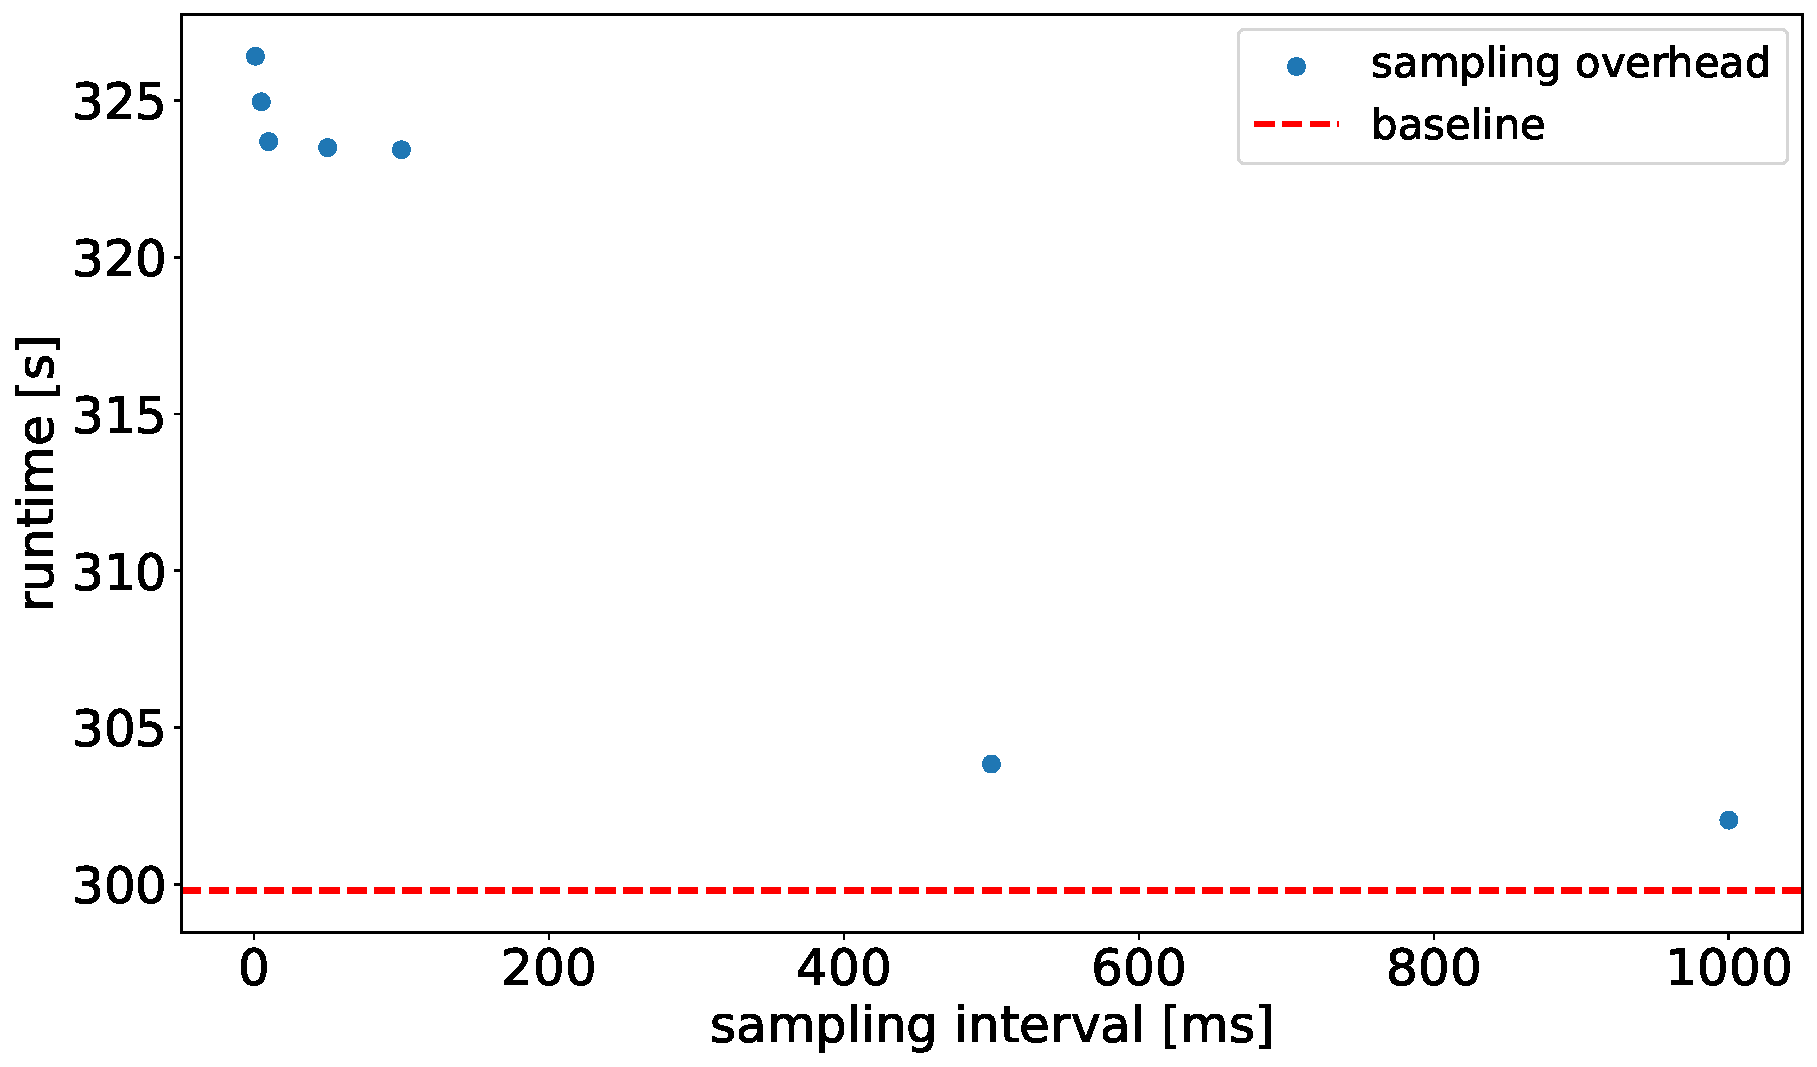
\includegraphics[width=0.8\linewidth]{figures/02_performance_portability/hws_sampling_interval_overhead}
    \caption{%
    The overhead when using the hws library, depends on the specified sampling interval. 
    The red dashed line at the bottom is the baseline version without hws. 
    We can see, that the overhead when using hws is noticeable for smaller sampling intervals. 
    However, increasing the sampling interval also drastically decreases the overhead. 
    }
    \label{fig:hws_overhead}
\end{figure}
\todo{remake plot (new runtimes with more data points)}

% \begin{figure}
%     \centering
    
%     \caption{%
%     The overhead when using the hws library, depends on the specified sampling interval. 
%     The red dashed line at the bottom is the baseline version without hws. 
%     We can see, that the overhead when using hws is noticeable for smaller sampling intervals. 
%     However, increasing the sampling interval also drastically decreases the overhead. 
%     }
%     \label{fig:hws_overhead}
% \end{figure}



\subsection{Hardware Sampling Implementation}

I have to differentiate the hws internal implementation targeting \glspl{cpu} and \glspl{gpu}.
To sample information on the supported \glspl{gpu}, I use the respective vendor-provided library. 
For NVIDIA \glspl{gpu} this is the \gls{nvml} library, for AMD \glspl{gpu} it is the \gls{rocmsmi} library, and for Intel \glspl{gpu} it is the Level Zero library. 
While the \glspl{api} are relatively similar for \gls{nvml} and \gls{rocmsmi}, Level Zero has a significantly different approach, which can also be seen in \autoref{code:vendor_library_calls}. 
Nevertheless, all functions are simple library calls.

On the \gls{cpu}, however, this is different since there is no simple library that I can call to gather all the necessary information. 
Here, I use three different command line utilities: to retrieve general \gls{cpu} information, like core-count, socket-count, cache-sizes, etc., I use \texttt{lscpu}~\cite{qian_lscpu_nodate}, for memory-related information, i.e., available, used, and total main memory, I use \texttt{free}~\cite{small_free_nodate}, and for everything else like frequency or power related information I use \texttt{turbostat}~\cite{brown_turbostat_nodate}. 
In all three cases, I create a new subprocess, call the respective utility, and then return the standard output as a string. 
This string contains all necessary information and is then post-processed to extract the data inside the \gls{cpu} hardware sampler. 
For \texttt{lscpu}, the subprocess simply calls \texttt{lscpu}. 
In the case of the \texttt{free} command, the command line flag \texttt{-b} is added to be sure that the memory size information is output in bytes. 
For \texttt{turbostat} it is a bit different. 
First, I have to note that to get the full \texttt{turbostat} information, it has to be called with root privileges. 
However, in newer \texttt{turbostat} versions, it is possible to get a subset of all possible information even if \texttt{turbostat} is not called with root privileges. 
I handle that distinction directly in CMake: it tests whether \texttt{turbostat} can be executed with root privileges and if this is not the case it tests whether it can be executed without root privileges. 
In the latter case, gathering information via \texttt{turbostat} is completely disabled. 
In the former case, I sample the information using the \texttt{turbostat} command \texttt{sudo turbostat -n 1 -i 0.001 -S -q} with \texttt{sudo} only present if \texttt{turbostat} can be executed with root privileges. 
This command samples all available information immediately (\texttt{-i 0.001}) exactly once (\texttt{-n 1}) and outputs the information in a short summary format (\texttt{-S}) skipping potential header information (\texttt{-q}). 
An example \texttt{turbostat} output with the mentioned command looks like displayed in \autoref{code:turbostat_output}. 

\begin{listing}
    \begin{minted}[fontsize=\setfontsize{6.5}]{text}
Avg_MHz  Busy%  Bzy_MHz  TSC_MHz  IPC   IRQ  POLL  C1   C2   POLL%  C1%   C2%     CorWatt  PkgWatt
39       1.77   2212     4686     0.92  818  1     156  819  0.01   3.03  110.73  4.58     264.06
    \end{minted}
    \caption{%
    An example output of the command \texttt{sudo turbostat -n 1 -i 0.001 -S -q} with root privileges enabled for \texttt{turbostat} on an AMD EPYC 9274F \gls{cpu}.
    }
    \label{code:turbostat_output}
\end{listing}
Note that the output of \texttt{turbostat} also depends on the used \gls{cpu}. 
For example, the output \autoref{code:turbostat_output} was gathered on an AMD EPYC 9274F \gls{cpu} and consists of $14$ table entries. 
If I run the same command for example on an Intel i5-10210U \gls{cpu}, the output consists of $52$ columns mostly adding more idle state information but also temperature-related information missing for the AMD \gls{cpu}.
